\documentclass[11pt]{scrartcl}
\usepackage[utf8]{inputenc}
\usepackage[sexy]{evanchen} 
\usepackage{graphicx}
\graphicspath{{8 Outsource K Math/Gambar/}}

\title{Pencacahan}
\author{Azzam and Akeyla}
\date{Maret 2023}

\begin{document}

\maketitle

\renewcommand*\contentsname{Daftar Isi}
\tableofcontents

\newpage

\section{Prinsip Dasar pada Kombinatorika}
\subsection{Prinsip Penjumlahan}
Apabila terdapat $a$ cara melakukan kegiatan $X$ dan $b$ cara melakukan kegiatan $Y$ serta kegiatan $X$ dan $Y$ tidak dapat terjadi secara bersamaan, maka terdapat $a + b$ cara untuk melakukan kegiatan $X$ ATAU $Y$.
\begin{example}
    Di sebuah warung, terdapat menu bakso dan mie ayam. Terdapat lima variasi bakso dan enam variasi mie ayam. Apabila seseorang ingin membeli satu makanan di warung ini, terdapat sebelas pilihan 
\end{example}

\begin{example}
    Tentukan banyak bilangan prima dua digit $n$ yang digit satuannya juga merupakan bilangan prima.
\end{example}

\begin{proof}[Solusi]
    Jika digit satuan dari $n$ merupakan bilangan prima, maka nilai digit satuan tersebut yang mungkin adalah $2, 3, 5,$ dan $7$. Kita akan menghitung banyak bilangan yang memenuhi syarat soal untuk setiap kemungkinan digit satuan tersebut.\\
    Jika digit satuan $n$ adalah $2$, maka $n$ genap dan otomatis akan habis dibagi oleh $2$ dan bukan bilangan prima. Sehingga, tidak ada solusi dalam kasus ini.\\
    Jika digit satuan $n$ adalah $3$, maka nilai $n$ yang memenuhi ada $6$, yakni $13, 23, 43, 53, 73,$ dan $83$.\\
    Jika digit satuan $n$ adalah $5$, maka $n$ akan habis dibagi oleh $5$ dan bukan bilangan prima. Sehingga, tidak ada solusi dalam kasus ini juga.\\
    Jika digit satuan $n$ adalah $7$, maka nilai $n$ yang memenuhi ada $5$, yakni $17, 37, 47, 67,$ dan $97$.\\
    Sehingga, total akan ada $5 + 6 = 11$ bilangan yang memenuhi syarat soal.
\end{proof}

Contoh sebelumnya merupakan salah satu contoh dari teknik bagi kasus.

\subsection{Prinsip Perkalian}
Apabila terdapat $a$ cara melakukan kegiatan $X$ dan $b$ cara melakukan kegiatan $Y$ serta pemilihan cara melakukan satu kegiatan tidak memengaruhi cara melakukan kegiatan lainnya, maka terdapat $a \times b$ cara untuk melakukan kegiatan $X$ DAN $Y$.

\begin{example}
    Di sebuah warung, terdapat sebelas pilihan makanan dan lima pilihan minum. Apabila seseorang ingin membeli satu makanan dan satu minuman di warung ini, terdapat $11\times 5 = 55$ pilihan
\end{example}

\begin{example}
    Banyak bilangan asli dua digit yang digit satuannya merupakan bilangan prima dan digit puluhannya merupakan bilangan ganjil adalah ...
\end{example}

\begin{proof}
    Nilai digit puluhan harus merupakan bilangan ganjil. Terdapat lima kemungkinan nilai digit ganjil ($1, 3, 5, 7, 9$).\\
    Nilai digit satuan harus merupakan bilangan prima. Terdapat empat kemungkinan nilai digit prima ($2, 3, 5, 7$). \\
    Sehingga banyak bilangan asli dua digit yang memenuhi syarat nilai kedua digit seperti pada soal adalah $5 \times 4 = 20$.
\end{proof}

\subsection{Prinsip Komplemen}
Apabila terdapat $a$ anggota di grup $X$ dan di antara anggota tersebut terdapat $b$ anggota $Y$ serta $Y$ merupakan bagian dari grup $X$, maka banyak anggota $X$ yang bukan $Y$ adalah $a - b$.

\begin{example}
    Apabila di sebuah warung terdapat $55$ kombinasi makanan dan minuman yang tersedia tetapi $10$ kombinasi yang ada tidak dapat dibeli karena kemahalan, maka hanya ada $55 - 10 = 45$ kombinasi makanan dan minuman yang dapat dibeli.
\end{example}

\begin{example}
    Banyak bilangan asli dua digit yang memuat setidaknya satu digit bilangan prima adalah ...
\end{example}

\begin{proof}
    Kita dapat menghitung persoalan ini dengan dua cara. Cara pertama adalah dengan membagi kasus berdasarkan letak digit bilangan prima di bilangan tersebut: puluhan atau satuan atau keduanya. \\
    Cara kedua adalah dengan menghitung komplemen. Yakni, bilangan dua digit yang tidak memuat digit bilangan prima. Dengan kata lain, bilangan dua digit yang kedua digitnya merupakan bilangan komposit. \\
    Digit komposit ada enam, yakni $0, 1, 4, 6, 8, 9$. Tetapi, digit $0$ tidak boleh dijadikan digit puluhan. Sehingga, banyak bilangan dua digt yang tidak memuat digit bilangan prima adalah $5 \times 6 = 30$.\\
    Secara keseluruhan, terdapat $90$ bilangan asli dua digit (Mengapa?). Sehingga, banyak bilangan dua digit yang memuat setidaknya satu digit prima adalah $90 - 30 = 60$.
\end{proof}

\subsection{Prinsip Inklusi-Eksklusi}
Diagram Venn. Sederhananya, $|A \cup B| = |A| + |B| - |A \cap B|$ dan $|A \cup B \cup C| = |A| + |B| + |C| - |A \cap B| - |B \cap C| - |C \cap A| + |A \cap B \cap C|$.

\begin{example}
    Di kelas, terdapat $27$ siswa. Sebanyak $15$ siswa suka bakso dan $18$ siswa suka mie ayam. Banyak siswa yang tidak suka keduanya adalah $3$ orang. Banyak siswa yang suka keduanya adalah ...
\end{example}

\begin{proof}
    $27 = 15 + 18 - x + 3$. Sehingga, $x = 9$. 
\end{proof}

\section{Latihan Prinsip Kombinatorika}

\begin{problem}
    Terdapat $20$ siswa di kelas. $12$ siswa memakai jam tangan. $10$ siswa memakai kacamata. Apabila banyak siswa yang tidak pakai jam tangan ataupun kacamata adalah $5$ maka banyak siswa yang pakai kacamata dan jam tangan sekaligus adalah ...
\end{problem}

\begin{problem}
    Merlin ingin pergi dari Medan ke Semarang dengan pesawat. Sayangnya, tidak ada penerbangan langsung dari Medan ke Semarang. Ada beberapa penerbangan dengan satu transit di Jakarta atau Batam. Diketahui ada $12$ pilihan penerbangan dari Medan ke Jakarta, $5$ pilihan dari Jakarta ke Semarang, $6$ pilihan dari Medan ke Batam, dan $4$ pilihan dari Batam ke Semarang. Banyak pilihan penerbangan yang dapat diambil Merlin adalah ...
\end{problem}

\begin{problem}
    Banyak string lima huruf yang semua hurufnya merupakan huruf vokal adalah ...
\end{problem}

\begin{problem}
    Banyak string lima huruf yang setidaknya salah satu hurufnya merupakan huruf vokal adalah ...
\end{problem}

% \begin{problem}
%     Banyak string lima huruf yang semua hurufnya merupakan huruf vokal dan tidak ada huruf yang berulang adalah ...
% \end{problem}

% \begin{problem}
%     Banyak tripel bilangan asli $(x, y, z)$ sedemikian hingga $x < y \leq 100$ dan $x < z \leq 100$ adalah ...
% \end{problem}

\begin{problem}
    (OSK 2022 Kemampuan Dasar) Banyaknya bilangan bulat dari $1001$ sampai $2022$ yang habis dibagi $15$ atau $9$ adalah ...
\end{problem}

\begin{problem}
    Semua susunan huruf-huruf yang terdiri dari 3 angka disusun. Jika AAA berada pada urutan pertama sedangkan AAB pada urutan kedua maka berada pada urutan berapakah susunan huruf OSN ?    
\end{problem}

\begin{problem}
    Banyak tripel bilangan asli $(x, y, z)$ sedemikian hingga $x < y \leq 100$ dan $x < z \leq 100$ adalah ...
\end{problem}

\begin{problem}
    Berapa banyak cara mengubini papan berbentuk seperti pada gambar \ref{bentukh} dengan tromino-L (gambar \ref{trominol})?
    \begin{figure}[h]
        \centering
        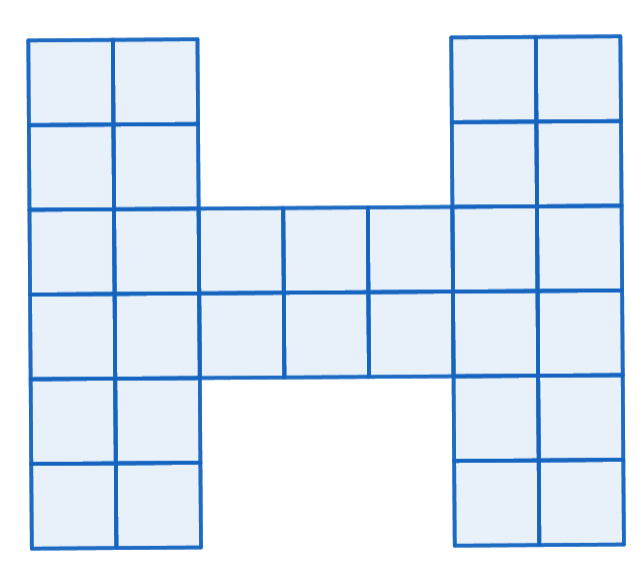
\includegraphics[width=0.5\linewidth]{bentukh.png}
        \caption{Papan yang ingin diubini}
        \label{bentukh}
    \end{figure}
    \begin{figure}[h]
        \centering
        \includegraphics[width=0.25\linewidth]{Trominol.png}
        \caption{Tromino-L}
        \label{trominol}
    \end{figure}
\end{problem}

\section{Permutasi dan Kombinasi}
\subsection{Permutasi}
Jika ada $n$ objek berbeda yang ingin diurutkan, banyak cara pengurutannya adalah \[n! = n\times (n - 1) \times (n - 2) \times ... \times 1\]
Jika ada $n$ objek berbeda dan terdapat pengulangan objek sebanyak $n_1$ objek pertama, $n_2$ objek kedua, dan seterusnya, maka banyak cara mengurutkan seluruh ibjek tersebut adalah \[\dfrac{n!}{n_1!n_2!...}\]
Jika ada $n$ objek berbeda dan akan dipilih $r$ objek di antaranya dengan memperhatikan urutan, banyak caranya adalah \[P_r^n = \dfrac{n!}{(n - r)!}\]

\begin{example}
    Ada $12$ belas orang siswa yang sedang berada di lorong sekolah. Mereka diminta untuk berbaris. Banyak cara mereka berbaris dapat dianggap sebagai permutasi $12$ objek berbeda yakni $12!$
\end{example}

\begin{example}
    Ada $5$ ekor kuda yang sedang balapan. Perankingan hanya dilakukan terhadap $3$ kuda tercepat. Yang ditanyakan adalah banyak kemungkinan urutan kuda ini di peringkat $3$ besarnya. \\
    Di sini, kita bisa memandang persoalan ini sebagai sebuah persoalan permutasi yang melibatkan $5$ objek (kuda) berbeda dengan $3$ objek (kuda) di antaranya akan dipilih dan memperhatikan urutan (melambangkan urutan podium kuda). Sehingga, banyak cara perankingannya adalah \[P_3^5 = \dfrac{5!}{(5 - 3)!}\]
\end{example}

\begin{example}
    Kita ingin menghitung banyak cara mengurutkan ulang kata $INDONESIA$. Di sini, kita tidak bisa secara langsung menghitung banyak huruf di kata ini dan kemudian menghitungnya dengan faktorial. Hal ini dikarenakan huruf $I$ dan $N$ muncul dua kali. Banyak huruf total adalah $9$ dan huruf $I$ serta $N$ muncul masing-masing dua kali. Artinya, banyak pengurutan ulang kata $INDONESIA$ adalah \[\dfrac{9!}{2!2!}\]
\end{example}

\subsection{Kombinasi}
Banyak cara memilih $r$ objek dari $n$ objek berbeda tanpa memperhatikan urutan adalah \[\binom{n}{r} = \dfrac{n!}{(n - r)!r!}\]

\begin{example}
    Banyak cara memilih $5$ dari $12$ siswa di kelas untuk dijadikan perwakilan kelas untuk lomba antarkelas adalah $\binom{12}{5} = \dfrac{12!}{7!5!}$
\end{example}

\subsection{Teorema Stars and Bars}
\begin{theorem}
    [Teorema Stars and Bars] Apabila terdapat sebuah persamaan bilangan cacah \[a_1 + a_2 + ... + a_r = n\] dengan $a_1, a_2,...,a_r, n, r$ merupakan bilangan cacah, maka banyak solusi $(a_1, a_2, ...,a_r)$ yang memenuhi adalah $\binom{n + r - 1}{r - 1}$.
    
    Jika $a_1, a_2, ..., a_r$ didefinisikan sebagai bilangan asli, maka banyak solusinya menjadi $\binom{n - 1}{r - 1}$
\end{theorem}

\begin{example}
    Banyak tripel bilangan cacah $x, y, z$ yang memenuhi persamaan $x + y + z = 10$ adalah $\binom{10 + 3 - 1}{3 - 1} = \binom{12}{2} = 66$
\end{example}

\begin{example}
    Banyak tripel bilangan \textbf{asli} $x, y, z$ yang memenuhi persamaan $x + y + z = 10$ adalah ...
\end{example}

\begin{proof}[Solusi]
    Perhatikan bahwa Teorema Stars and Bars hanya bisa dipakai apabila variabelnya merupakan bilangan cacah dan bukan bilangan asli. Meskipun begitu, kita dapat mentransformasikan nilai $x, y, z$ ke bilangan cacah. Yakni, dengan mendefinisikan $a = x - 1, b = y - 1, c = z - 1$. Sekarang, $a, b, c$ adalah bilangan cacah. Substitusikan ini ke persamaan awal dan diperoleh $a + b + c = 7$. Dengan Stars and Bars, diperoleh banyak solusinya adalah $\binom{7 + 3 - 1}{3 - 1} = \binom{9}{2} = 36$
\end{proof}

\section{Latihan Permutasi dan Kombinasi}
\begin{problem}
    Tentukan banyak cara mengacak huruf-huruf di kata-kata berikut:
    \begin{enumerate}[i.]
        \item OSN
        \item MEDAN
        \item JAKARTA
        \item BOJONGSOANG
    \end{enumerate}
\end{problem}

\begin{problem}
    Diberikan sekumpulan huruf: $\{A,C,E,I,K,L,S\}$. Dengan menggunakan kumpulan huruf ini,
    \begin{enumerate}[i.]
        \item Ada berapa banyak "kata" $5$ huruf dengan huruf yang dipakai boleh diulang?
        \item Ada berapa banyak "kata" $5$ huruf dengan huruf yang dipakai tidak boleh diulang?
        \item Ada berapa banyak "kata" $7$ huruf dengan huruf yang dipakai boleh diulang?
        \item Ada berapa banyak "kata" $7$ huruf dengan huruf yang dipakai tidak boleh diulang?
        \item Ada berapa banyak "kata" $7$ huruf, tidak ada huruf yang boleh diulang, dan huruf vokal dan konsonan harus berada secara berseling-seling?
        \item Ada berapa banyak "kata" $7$ huruf, tidak ada huruf yang boleh diulang, dan tidak memuat subkata "AK"?
    \end{enumerate}
\end{problem}

\begin{problem}
    Ada $12$ orang pada suatu kelas, $5$ di antaranya perempuan. Tentukan banyak cara menyusun $12$ orang tersebut pada satu baris, jika:
    \begin{enumerate}[i.]
        \item Tidak ada syarat
        \item Kelima perempuan harus duduk bersebelahan
        \item Laki-laki dan perempuan duduk terpisah
        \item Tidak boleh ada dua perempuan yang duduk bersebelahan
        \item Di antara Aji dan Bobi (dua laki-laki di kelas tersebut) tidak ada laki-laki tetapi ada tepat tiga orang perempuan.
    \end{enumerate}
\end{problem}

\begin{problem}
    (AMC 10B 2018) Tentukan banyak himpunan bagian dari $\{2, 3, 4, 5, 6, 7, 8, 9\}$ yang memuat setidaknya satu bilangan prima.
\end{problem}

\begin{problem}
    Seekor semut yang berada di titik $(0, 0)$ ingin menuju ke titik $(5, 5)$. Dalam satu langkah, semut tersebut hanya bisa berpindah ke kanan sejauh satu satuan atau ke atas sejauh satu satuan. Banyak urutan langkah berbeda yang semut tersebut ambil adalah ...
\end{problem}

\begin{problem}
    (AMC 10A 2007) Enam orang turis sedang berwisata dipandu oleh dua orang pemandu. Dikarenakan medan yang sempit, kedelapan orang ini dipisah menjadi dua rombongan. Setiap orang memuat satu pemandu dan setidaknya satu turis. Banyak cara membagi kedelapan orang ini adalah ...
\end{problem}

\begin{problem}
    \begin{enumerate}[i.]
        \item Enam siswa laki-laki dan enam siswi perempuan akan menari secara berpasangan. Setiap pasangan berisi satu laki-laki dan satu perempuan. Banyak cara membentuk enam pasangan tari ini adalah ...
        \item Ternyata, setelah diadakan simulasi tari, Rahmat (laki-laki) dan Lestari (perempuan) harus berpasangan sedangkan Erlangga (laki-laki) dan Erika (perempuan) tidak bisa berpasangan. Banyak cara membentuk pasangan tari dengan syarat ini adalah ...
    \end{enumerate}
\end{problem}

\begin{problem}
    (HMMT Kombinatorika Februari 2013) Berapa banyak permutasi dari $(a_1, a_2,..., a_8)$ dari $\{1, 2, 3,..., 8\}$ yang memenuhi $a_1 - a_2 + a_3 - a_4 + a_5 - a_6 + a_7 - a_8 = 0$?
\end{problem}

\begin{problem}
    Ada $12$ permen yang akan dibagikan ke $3$ orang. Berapa banyak cara membagi permen ini apabila:
    \begin{enumerate}[i.]
        \item Setiap permen identik dan setiap orang harus mendapatkan banyak permen yang sama
        \item Setiap permen identik dan banyak permen yang didapat setiap orang boleh berbeda (dan boleh nol)
        \item Setiap permen dianggap berbeda dan banyak permen yang didapat setiap orang boleh berbeda (dan boleh nol)
        \item Setiap permen dianggap berbeda dan setiap orang harus mendapatkan banyak permen yang sama
    \end{enumerate}
\end{problem}

\begin{problem}
    (HMMT Kombinatorika Februari 2014) Hitunglah banyak tripel himpunan $(A, B, C)$ yang memenuhi:
    \begin{enumerate}
        \item $A, B, C \subseteq \{1, 2, 3, ..., 8\}$ 
        \item $|A \cap B| = |B \cap C| = |C \cap A| = 2$
        \item $|A| = |B| = |C| = 4$
    \end{enumerate}
\end{problem}
\end{document}